\section{K\_W15, K\_W03, K\_W04, K\_W07, K\_U15, K\_U21, K\_U22, K\_U03, K\_U04}
\textbf{304. $\varepsilon$-domknięciem E dla stanu początkowego $q_1$ dla przedstawionego ponizej automatu są zbiory}

\begin{figure}[h!]
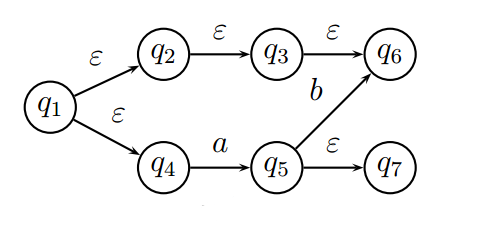
\includegraphics[scale=0.5]{automata.png}
\end{figure}

przykładowa odp.) $E(q_1) = \emptyset$; – tj. nie da się wyznaczyc ze względu na puste przejścia\\
\textbf{FAŁSZ}\\\\

$\varepsilon$-domknięcie stanu $q E(q)$ definiuje się:
\begin{enumerate}
\item Podstawa: Stan $q$ należy do $E(q)$
\item Krok indukcyjny: Jeżeli stan $p$ należy do $E(q)$ oraz istnieje przejście ze stanu $p$ do stanu $r$ o etykiecie $\varepsilon$, to $r$ należy do $E(q)$ - jeżeli funkcją przejścia opisywanego NAS jest $\delta$ i $p$ należy do $E(q)$, to $E(q)$ zawiera także stany z $\delta(p, \varepsilon)$.
\end{enumerate}

Dla zadanego automatu $E(q) = \{q_1, q_2, q_3, q_4, q_6\}$
